\section{Communications}
\label{blDOCOM}

For the communications subsystem 5 different topics were investigated:
\begin{itemize}
\item Tracking
\item Swarm satellites crosslink frequency
\item D/L and U/L frequency
\item Antenna configuration
\item Communications architecture
\end{itemize}

\subsection{Tracking}
For tracking there are the following design options:
\begin {itemize}
\item \ac{MANS}
\item \acs{GPS}
\item \ac{TDRS}
\item Satellite crosslinks
\item Ground tracking
\end {itemize}

MANS uses observations of the Earth, Sun and Moon from a single sensor to provide real-time position and attitude data. These objects can be unambiguously identified with high reliability and low cost. Observations can be done with minor modifications to attitude sensors which are already on most spacecraft. The MANS flight software can also make use of data from a GPS receiver, star sensors, gyros and accelerometers to increase the accuracy. MANS can provide ground point look and sun directional information, which also works at any altitude in between \acs{LEO} and \acs{GEO}.

GPS is a system of navigation satellites which allows position determination with an accuracy of 50-100 m for non-military use. GPS can also be used to determine attitude by using multiple GPS antennas attached to a rigid element of the spacecraft which allows accuracies between 0.3 and 0.5 degrees. There must always be four GPS satellites in sight in order for the system to work, but which can not be guaranteed that this number of satellites is in sight continuously.

TDRS is a system of two satellites operated by NASA, which can provide tracking data coverage of 85\% to 100\% of most low-Earth orbits. The system collects mostly range and range-data from the TDRS satellite to the satellite being tracked. Angular information is available, but which is much less accurate than the range and range-rate data. If atmospheric drag effects on a satellite are small, TDRS can achieve 3$\sigma$ accuracies of 50 m, which is considerably better than most ground-tracking systems.

Satellite crosslinks allow relative position determinations by using of cross link equipments. If absolute position determination is required, a separate tracking system is required. Which can also allow relative position determination, making the satellite crosslinks technique redundant.

Finally ground tracking allows determination of range and range rate. Angular measurements are also available at times but which are typically far less accurate. Several passes over a ground station are required for orbit determination. 3$\sigma$ accuracies typically are about several kilometers for \ac{LEO}.

\subsection{Swarm Satellites Crosslink Frequency}
The frequency band normally used for inter satellite communications are the V-band frequency. This band lies around 60 GHz and has no limit on the power flux density.

\subsection{D/L and U/L Frequency}
Frequency bands available for upload and download of scientific data are:
\begin{itemize}
\item C-Band
\item X-Band
\item Ku-Band
\item Ka-Band
\item SHF/EHF-band
\end{itemize}

Details for all frequency bands can be found in \cite{larson}, p. 566.

\subsection{Antenna Configuration}
The following antennas, suitable for beamwidths of less than 20 degrees, producing gains above 15dB, are considered:
\begin{itemize}
\item Parabolic reflector center-feed
\item Parabolic reflector cassegrain
\item Parabolic reflector off-set feed
\item Phased array
\item Lens with switched-feed array
\item Parabolic reflector off-set shaped subreflector with feed array for scanning
\end{itemize}

Drawings and descriptions of these antennas can be found in \cite{larson}, p. 573.

\subsection{Data Storage}
Today Dynamic RAM is almost exclusively used by satellites for mass data storage because they allow very large capacities of 1000 Gbits and more. Typically, they do not have external addressing to each RAM location but operate on a block or file basis. The block may be of the order of 1000 bytes or sometimes it will correspond to one source packet. Dynamic RAM has a simple structure: only one transistor and a capacitor are required per bit, compared to six transistors in Static RAM. This allows Dynamic RAM to reach a very high density \cite{sse}.

Since this technology has recommended itself as the best around, there is no logical reason to design or trade-off other options. For this reason it is not included in the design option tree.

\subsection{Communications Architecture}
In this subsection we will discuss the possible communications architectures and the transmission power and bandwidth required for the communication subsystem in each satellite:
\begin{itemize}
\item Centralized architecture
\item Decentralized architecture
\item Extremely decentralized architecture
\end{itemize}

In centralized architecture there is one central satellite which handles all communication between the swarm and the Earth. Which means the communication subsystem of the central satellite requires a broad bandwidth and high transmission power both for the communication between itself and the swarm and the Earth. All data can be stored, organized and compressed efficiently on this central satellite. Data can also be stored on each satellite as a backup in case there is no continuous communication.

A decentralized architecture gives all satellites the bandwidth and transmission power to communicate with the ground, but communication within the swarm is also still possible. In this architecture each satellite has to store its own data itself.

In an extremely decentralized architecture all satellites communicate independently to the ground and also communication between the swarm goes through ground stations. Also for this architecture all satellites need to store their own data.

The design option tree for communications subsystem is shown in figure \ref{fig:DOCom} on page \pageref{fig:DOCom}.

\begin{figure} [ht!]
	\centering
	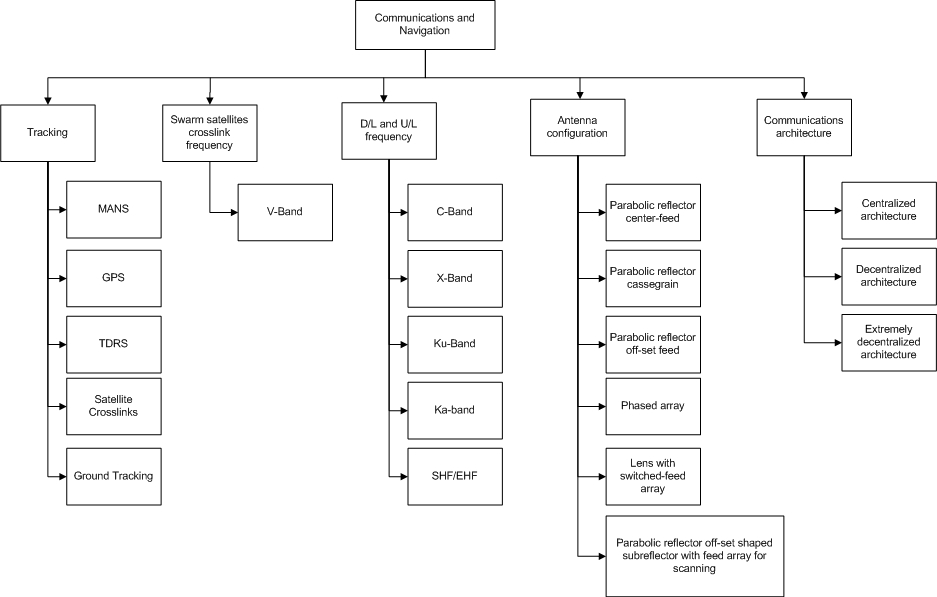
\includegraphics[width=0.9\textheight,angle=90]{chapters/img/DOTCom.jpg}	
	\caption{Design option tree for communication systems}
	\label{fig:DOCom}
\end{figure}
